\chapter{Hauptteil/Main Part}




\section{Hardware Reference}

\begin{table}[h!]
    \centering
    \begin{tabular}{|l|c|p{5cm}|}
        \hline
        \textbf{Basic Component List} & \textbf{Number} & \textbf{Notes} \\
        \hline
        NodeMCU ESP32  & 1 & Development board for prototyping \\
        \hline
        1,8" LCD Display Module  & 1 & 128x160 Pixel, ST7735R (Display Driver), includes microSD Slot \\
        \hline
        Button module with 2 Buttons & 1 & For interacting \\
        \hline
		Jumper Wires Female to Male & 22 & For connecting components \\
        \hline
        Breadboard & 1 & For building circuits \\
        \hline
    \end{tabular}
    \caption{Basic Component List for Guardian Prototype}
    \label{tab:basic-component-list}
\end{table}

\begin{figure}
	\centering
	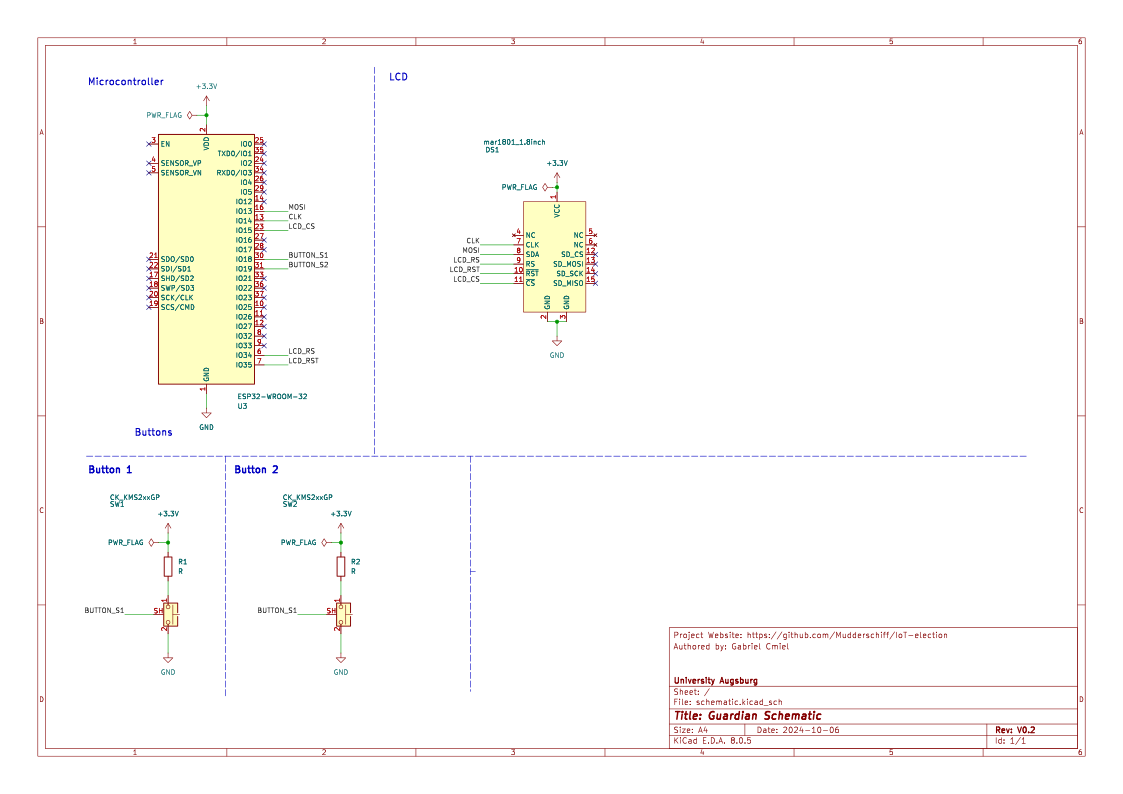
\includegraphics[scale=.5]{abbildungen/schematic.png}
	\caption{Schematic of the Guardian Prototype}
	\label{Fig:schematic}
\end{figure}

As shown in Table \ref{tab:basic-component-list}, the hardware components used in our prototype include a ESP32 development board, an LCD display module, jumper wires, breadboard and a module with 2 Buttons. The connectivity of these components are shown in the schematic in Figure \ref{Fig:schematic}. The NodeMCU ESP32 development board is used as the Main Controller. The LCD display module is used to display information to the user. The button module is used to interact with the user. The jumper wires are used to connect the components. The breadboard is used to build the circuits.

\subsection{NodeMCU ESP32 Development Board}
The NodeMCU ESP32 development board is equipped with the ESP32-WROOM-32 module. The ESP32-WROOM-32 module is a powerful, generic Wi-Fi+Bluetooth+Bluetooth Low Energy MCU module. At the core of this module is the System on a Chip (SoC)ESP32-D0WDQ6. \cite[6]{esp32-module}. The ESP32-D0WDQ6 chip is based on chip revision v.1.0 or v1.1. \cite[11]{esp32-ds}. The ESP32-WROOM-32 module could therefore be replaced by the newer ESP32-WROOM-32E module. The ESP32-WROOM-32E module uses a ESP32-D0WD-V3 or ESP32-D0WDR2-V3 chip which are based on chip revision v3.0 or v3.1 which fixes some Hardware bugs \cite[1]{esp32-module-new}, \cite[11]{esp32-ds}, \cite[3-4]{esp32-errata}. 

\subsection{1,8" LCD Display Module}
The 1,8" LCD Display Module has a resolution of 128x160 Pixels and is equipped with a ST7735R Display Driver.  The module also contains a microSD Slot which won't be used in this project \cite[2]{lcd}.
The ESP-IDF component lvgl_esp32_drivers


\subsection{Button Module}
The Button Module is an integrated circuit that features 2 buttons and integrated pull-up resistors. \cite[1]{button-ds}


\section{Implementation}
\subsection{Python Client}
Our python client imports the python package ElectionGuard \cite{python-reference}. The ElectionGuard Python package is a reference implementation of the ElectionGuard 1.0 specification. It covers the entire suite of functionality required to implement an end-to-end verifiable election as part of a voting system \cite{eg-docs}. 



In the proposed voting system the python client will act as the administrator, the ballot box and the encryption device of the election. Administrating the election requires loading and semantically verifiying the Election manifest before the election.





Before the election the python client load the Election Manifest for our election and semantically checks the data format required to conduct an ElectionGuard Election. 




The python client loads the manifest file used for our election. In ElectionGuard an election manifest has to be semantically checked against the data format required to conduct an ElectionGuard Election. 


The python client then generates the election keys and the election context. The election keys are used to encrypt the ballots and the election context is used to verify the election. The python client then encrypts the ballots and generates the proofs of the encryption. The encrypted ballots and the proofs are then sent to the ESP32. The ESP32 decrypts the ballots and verifies the proofs. The ESP32 then generates the proofs of the decryption and sends them back to the python client. The python client then verifies the proofs of the decryption and generates the proofs of the election. The proofs of the election are then sent to the ESP32. The ESP32 verifies the proofs of the election and sends the results back to the python client. The python client then verifies the results and outputs the final results of the election.

The tasks of the python client can be divided into three stages pre-election, intra-election and post-election.







The python client loads the manifest file used for our election. In ElectionGuard an election manifest has to be semantically checked against the data fromat required to conduct an ElectionGuard Election.



Espressif IoT Development Framework (ESP-IDF) is a software development framework intended for the development of Internet-of-Things (IoT) applications for the ESP32 board \cite[3]{esp-idf}. ESP-IDF consists of components written specifically for ESP-IDF as well as third-party libraries.\cite[123]{esp-idf} For example, the real-time operating system kernel used for ESP-IDF applications is the third-party component called FreeRTOS \cite[1893]{esp-idf}. ESP-IDF projects use the same componment based approach and can be seen as an amalgamation of a number of components \cite[2240]{esp-idf}.

\begin{figure}
	\centering
	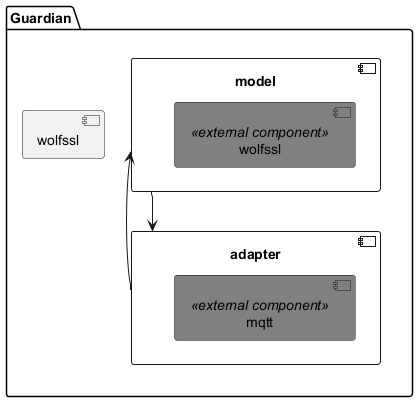
\includegraphics[width=1\textwidth]{abbildungen/Diagramme/components.png}
	\caption{}
	\label{Fig:uml-classes-python}
\end{figure}



ESP32 contains a hardware random number generator, values from it can be obtained using the APIs 'esp_random()' and 'esp_fill_random()'. If certain conditions are met, the RNG mixes samples of physical noise continously into the internal hardware RNG state to provide entropy. If the conditions are not met, the output of the RNG should be considered pseudo-random. \cite[2140]{esp-idf}


\subsection{Model}
\begin{figure}
	\centering
	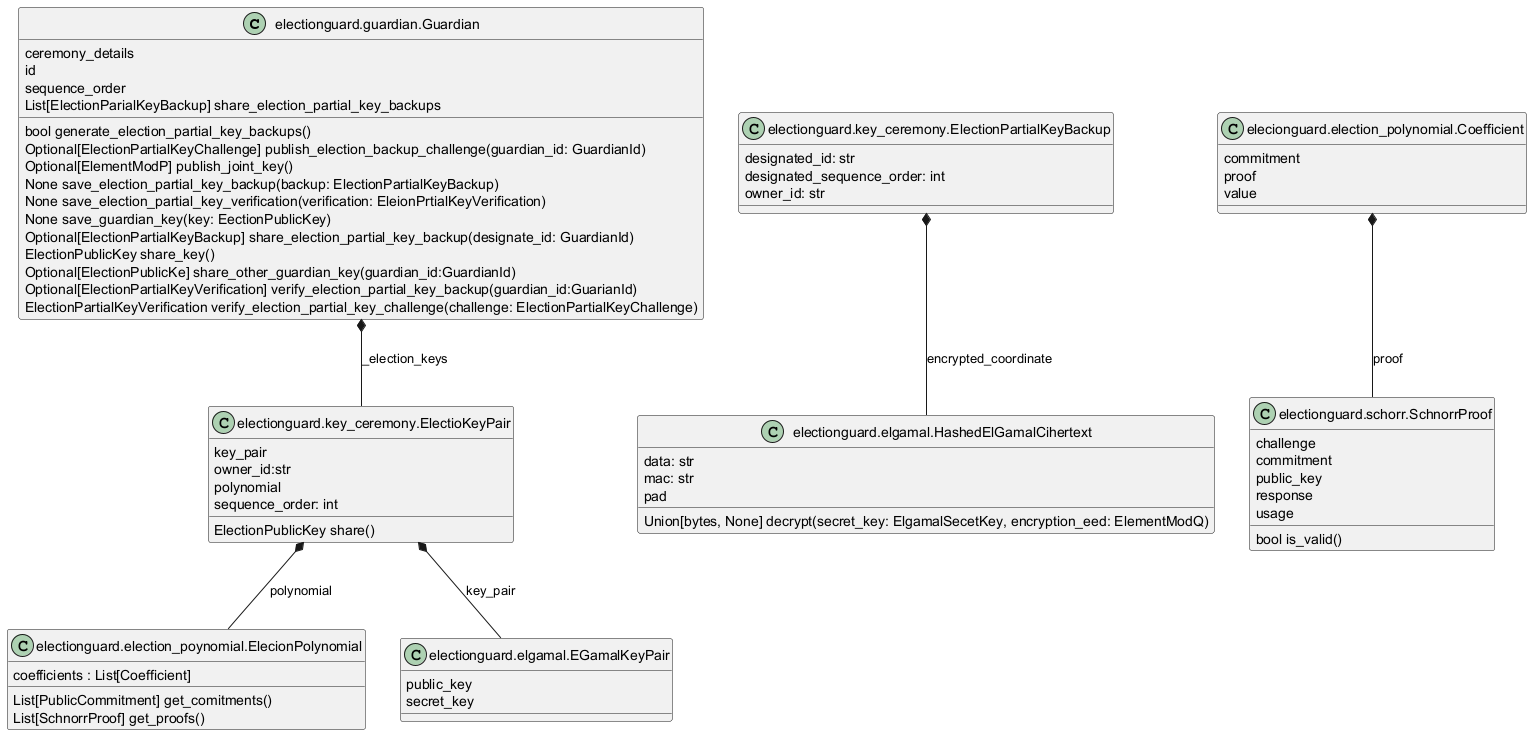
\includegraphics[width=1\textwidth]{abbildungen/Diagramme/python-classes.png}
	\caption{Selected Python Classes from Reference Implementation for Guardian Functionality}
	\label{Fig:uml-classes-python}
\end{figure}

ElectionGuard uses integer ElGamal within specific cryptographic equations three large integer operations are often performed all on very large integer values. These operations are modular exponentiation, modular multiplication, and modular addition. These operations can be performed by either importing specialiced tools to perform these large integer operations, or by implementing these operations from scratch. When implementing these operations from scratch, intermediate values can get excessively large often times it is necessary to perform special methods such as modular reduction to keep the values within a reasonable range.  \cite[21, 25-26]{eg-spec}. Another important operation within ElectionGuard is SHA-256 hash computations. 

\subsubsection{Comparison with other Implementations}
The modular exponentiation operation imposes the highest computational cost among all computations and is the limiting factor in any performance analysis. \cite[22]{eg-spec}. Using fast libraries for modular arithmetic is thus crucial to achieve good performance \cite[22]{eg-paper}. The Python reference implementation of ElectionGuard uses the C-code Gmpy2 library for large integer arithmetic. \cite{eg-docs}. \cite{esp32-ref} The C++ and Kotlin implementations of ElectionGuard uses HACL* C library for cryptographic primitives. \cite{eg-docs}. Furthermore, the C++ implementation also uses pre-computed tables to speed up some modular exponentiations \cite{eg-docs}. This is possible because most exponentiations have a fixed base, either the constant generator or the election public key. The pre-computed tables contain certain powers of these bases. \cite{eg-docs}.

\subsection{Feasability of the Python reference on ESP32}
It could be possible to run the python reference on the ESP32 using Micropython. Micropython is an implementation of Python 3.x targetting microcontrollers and embedded systems. Functionalities of the python standard library are mirrored and "micro-ified" to fit with the limitations of microcontrollers such as memory and speed \cite{micropython} \cite[234]{9292199}. Apart from python the electionguard python reference requires the C-coded python library Gmpy2 for large integer arithmetic \cite{eg-ref}. Disadvantages of this approach is that some needed modules, functions and classes may be missing from Micropython. \cite{micropython}. Furthermore, MicroPython applications suffer from memory fragmentation and objects that grow in size \cite[234]{9292199}. Depending on task complexity and memory allocation MicroPython performs lower than the C implementation \cite[237]{9292199}. In a comparison of software based SHA-256 computation for the ESP32 the C implementation was faster than the MicroPython implementation by 45\% \cite[237]{9292199}. 

\subsection{Feasability of the C++ reference on ESP32}
ESP32 supports development of applications in C++. The ElectionGuard C++ implementation uses exception handling. C++ Exception handling has to be enabled in ESP-IDF. This will increase the application binary size by a few KB. Runtime Type Information (RTTI) can be left disables as dynamic cast conversion and the typeid operator are not used in the ElectionGuard C++ implementation. ESP32 also supports C++ threads however these are wrappers around C pthreads which in turn wrap FreeRTOS tasks. \cite{espidf-docs}. After porting the C++ implementation into an ESP32 component we test the component using the included C Unit Tests specifically the test for elgamal encryption. The test crashes after calling pow_mod_p(). pow_mod_p() is a function to speed up modular exponentiation by using a fixed-base lookup table. 

\begin{lstlisting}[language=C++, caption={FixedBaseTable Definition}]
    typedef std::array<std::array<uint64_t[MAX_P_LEN], OrderBits>, TableLength> FixedBaseTable;
\end{lstlisting}

The FixedBaseTable is a 2d Array. MAX_P_LEN is the length of each uint64_t array. OrderBits is the number of uint64_t arrays in each inner array. TableLength is the number of inner arrays in the outer array. 


The pow_mod_p() implementation is tuned specifically for the following values: b order bits = 256, k window size = 8, m table length = 32. Any changes to these values may impact the internal operation of the functions. The Window Size determines to parse the exponent into groups of k bits. The Order Bits represents the number of of possible values in each group. For an 8-bit windows size the orderbits would be 256 (2^8) \cite[22]{eg-spec}. The total size in bytes of the FixedBaseTable can be calculated as follows:

\begin{equation}
    \text{FixedBaseTable Size} = \text{sizeof(uint64\_t)} \times \text{MAX\_P\_LEN} \times \text{OrderBits} \times \text{TableLength}
\end{equation}
MAX_P_LEN is defined as 64. Substituting the above equation with the actual values we get 4MB.

\begin{equation}
    \text{FixedBaseTable Size} = 8 \times 64 \times 256 \times 32 = 4194304 \text{ bytes} = 4 \text{ MB}
\end{equation}

If we calculate the size of the FixedBaseTable with the reduced baseline parameters

\begin{equation}
    \text{FixedBaseTable Size} = 8 \times 48 \times 256 \times 32 =  3145728 \text{ bytes} = 3 \text{ MB}
\end{equation}

The ESP32 has 320KB of DRAM to hold data. Due to a technical limitation the maximum memory available for dynamic allocation is 160KB. \cite{esp32-ref}. This means that the FixedBaseTable is too large to be stored in the ESP32's memory. A decrease in window size k leads to smaller tables and thus less memory usage, but increases the number of multiplications. \cite[22]{eg-spec}. The ElectionGuard C++ implementation assumes Intel Atom class processor level performance and Raspberry Pi3 types of operating systems \cite{eg-docs}. Base on these assumptions and the memory usage of the FixedBaseTable the ElectionGuard C++ implementation is not feasible on the ESP32.

\subsection{C Implementation}
From the previous sections we know that running both the Python and C++ reference implementations on the ESP32 is not feasible. In the case of Python there is the issue of possible memory fragmentation and performance and in the case of the C++ implementation the high memory requirements. Furthermore, the C++ implementation only contains the encryption library and thus only contains the intra-election steps as outlined in the background chapter. Interestingly, both implementations use a C coded library for modular arithmetic. For these reasons the author opts for a pure C implementation on the ESP32. 

\subsubsection{Performance of Cryptographic Operations}
It is essential to test if the cryptographic algorithms used are viable in terms of execution time and memory consumption.

\begin{figure}
	\centering
	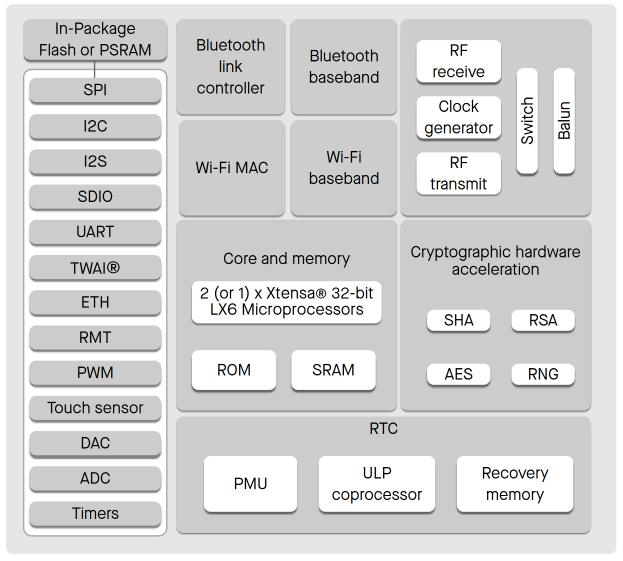
\includegraphics[scale=.5]{abbildungen/functional-block-diagram}
	\caption{ESP32 Functional Block Diagram}
	\label{Fig:esp32-crypto}
\end{figure}
As seen in the Functional Block Diagram of the ESP32 \ref{Fig:esp32-crypto} the ESP32 is equipped with Cryptographic hardware acceleration for general algorithms such as AES, SHA, RSA. The SHA Accelerator supports four algorithms: SHA-1, SHA-256, and SHA-384, and SHA-512. 

The SHA Accelerator requires 60 to 100 clock cycles to process a message block and 8 to 20 clock cycles to calculate the final hash. For SHA256 a message block is 512 bits. The Accelerator only accepts one message block at a time furthermore the accelerator is unable to perform padding operations. Thus User software is expected to divide longer messages into 512-bit blocks and perform padding operations if needed. \cite[2]{esp32-ds}. The performance of SHA-256 with the SHA Accelerator and with a CPU frequency of 240MHz is 181.3\% higher than without the SHA Accelerator. \cite[41]{performance-evaluation}. The performance is nearly 3 times faster with hardware acceleration compared to without. \cite[41-42]{performance-evaluation}.



Comparing the throughput performance of the SHA-256 with and without the SHA Accelerator the SHA Accelerator is has a 181.3%





hardware accelerators of general algorithms, such as AES, SHA, RSA, and ECC. \cite[2]{esp32-ds}


libraries
mbedtls: C library that implements cryptographic primitives
Graphics Library: lvgl
Communication: protobuf for serialization





\subsection{Adapter}
The under-specification 

\subsection{View}





Abkürzungen müssen im Abkürzungsverzeichnis angelegt werden.
Erste Verwendung einer \ac{ABK} jede weitere Verwendung der \ac{ABK}.

%Befehl um sämtliche Literatur im Literaturverzeichnis aufzuführen
\nocite{*}

